\chapter{Idémyldring}
I dette steget av prosessen er målet å generere en liste over det vi tror kan være mulige årsaker til problemet. Det er en del forskjellige verktøy en kan bruke for å oppnå dette, men vi har valgt å benytte Idémyldring på basis av RCA boken \cite{RCA} sin fremgangsmåte for valg av verktøy.

\section{Idémyldring}
Med rotårsaksanalyse finnes det to ulike måter å gjennomføre idémyldring på: strukturert- og ustrukturert idémyldring. I den strukturerte versjonen får hver deltaker sin tur til å komme med en idé, og dette sikrer at alle får delta like mye. På den ustrukturerte måten kan alle komme med idéer etterhvert som de kommer på dem, og fungerer mye mer spontant enn den strukturerte. Det er spesielt viktig å ikke omformulere eller diskutere forslagene etterhvert som de kommer, dette skal gjøres etter idémyldringsøkten er over.

\subsection{Ønsket utbytte}
Ønsket utbytte ved å bruke idémyldring er å få en forståelse av hva som kan være rotårsaken til at NTNU sine ressurser blir misbrukt til utvinning av kryptovaluta. Vi ønsker også å skape et godt grunnlag av idéer som kan brukes i datainnsamling i neste del av oppgaven.

\subsection{Gjennomføring}
Vi startet idémyldringen med å finne ut hva som burde fokuseres på av hvordan og hvorfor skolen sine ressurser blir missbrukt til utvinning av kryptovaluta. Vi kom frem til at begge deler var like viktige, og at vi burde ha to idémyldringer for å komme med flest mulige idéer som ville kunne hjelpe oss i hva som burde spørres om i datainnsamlingen. De to ``basene'' til idémyldring vi brukte i idémyldringsprossesen var: hvordan eller hvorfor ``blir NTNU sine ressurser missbrukt i utvinning av kryptovaluta''. Idémyldring prosessen var litt annerledes enn de vi hadde i de andre oppgavene, der vi denne gangen hadde et mer idéskrivingsoppsett, der vi alle skrev inn de idéene vi hadde inn i et dokument.

\subsection{Resultater}
Etter at økten var ferdig ble det gjort en vurdering av hvilke momenter som hørte sammen eller hadde likhetstrekk og disse ble gruppert, se figur \ref{fig:idemyldring-hvordan} og \ref{fig:idemyldring-hvorfor} under.


%Dette kan være ved hjelp av script som miner mens en intern er på nettsiden eller annen skadevare.


\begin{figure}[H]
    \centering
    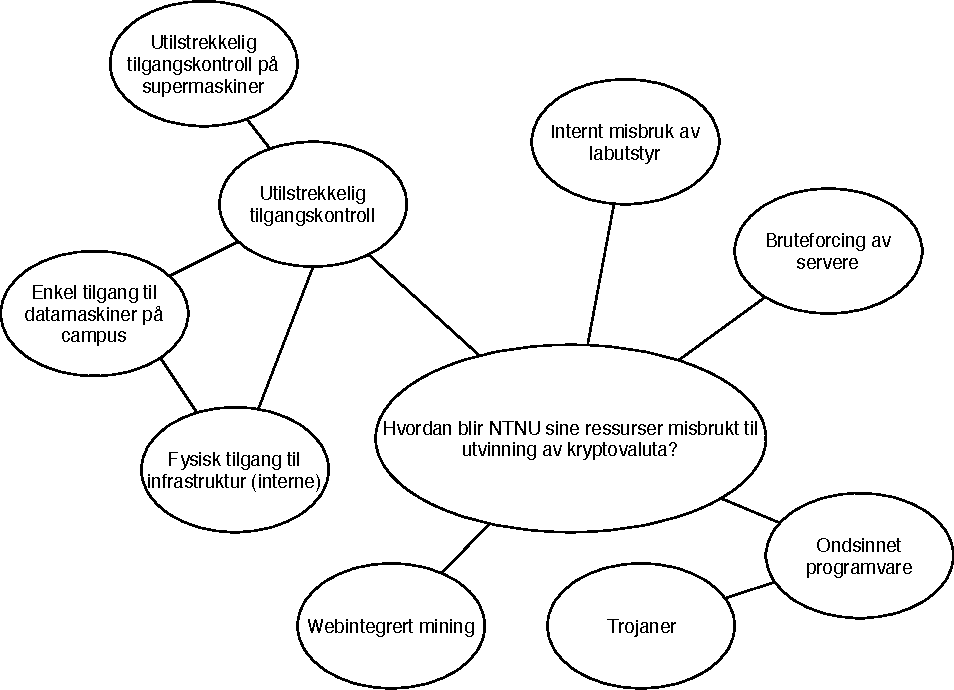
\includegraphics[scale=0.5]{case_3/bilder/idemyldring-hvordan.pdf}
    \caption[Idémyldring]{Resultater og gruppering av Hvordan}
     \label{fig:idemyldring-hvordan}
\end{figure}

\begin{figure}[H]
    \centering
    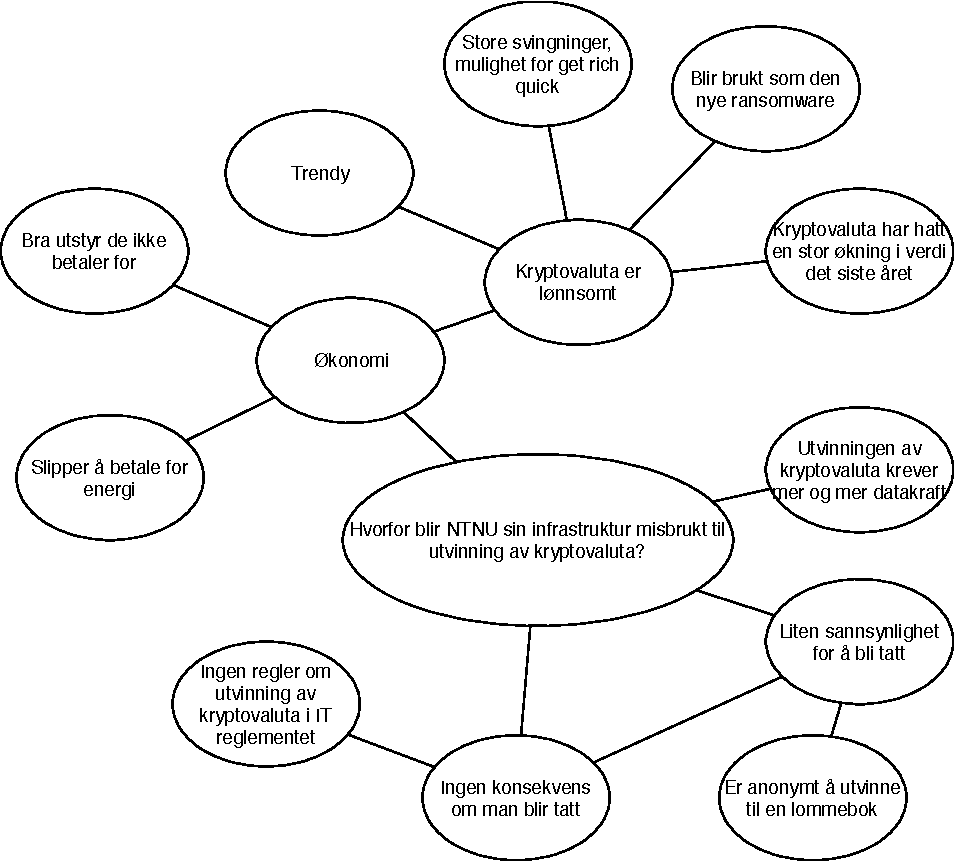
\includegraphics[scale=0.5]{case_3/bilder/idemyldring-hvorfor.pdf}
    \caption[Idémyldring]{Resultater og gruppering av Hvorfor}
    \label{fig:idemyldring-hvorfor}
\end{figure}

RESULTAT

\subsection{Konklusjon av verktøyet}
Verktøyet hjelper til med å få økt forståelse på hva som er årsaker til problemstilingen eller i denne samenheng to problemstilinger. Finnes det en klar problemstiling er det lett å komme med ideer på hva som er årsakene. Det gir et god overordnet bilde av situasjonen, men siden vi har lite tid på dette caset kommer det veldig mange idéer, der noen trolig blir unødvendige å følge.

\section{Nominell gruppeteknikk}
Nominell gruppeteknikk anbefales dersom det er idéer som må prioriteres. 

\subsection{Ønsket utbytte}
Ettersom vi har dårligere tid på dette caset enn på de tidligere, har vi valgt å benytte NGT for å prioritere idéer. NGT er også et verktøy vi er interessert i å prøve ut for hovedrapporten.

\subsection{Gjennomføring}
NGT ble utført med at vi alle satt oss ned sammen og hadde 15 poeng hver å gi til forskjellige idéer. Idéene ble laget utifra forarbeidet som var blitt gjort i idémyldringsprosessen, de idéene som lignet på hverandre ble slått sammen og noen ble litt omformulert. Idéene skulle få poengene 1, 2, 3, 4 eller 5 og alle disse 15 poengene skulle gis ut. Hver person ga ut sine 15 poeng for hva de trodde ville være det viktigste å fokusere på videre i analysen, og disse dataene kan sees i tabell \ref{tab:NGT}.

\subsection{Resultater}
Etter at hvert gruppemedlem hadde gitt ut sine 15 poeng satt vi igjen med 4 idéer som stakk seg ut med hvor mange poeng de fikk, disse er i fet skrift i tabell \ref{tab:NGT}. Disse fire årsakene er de vi kommer til å fokusere på i dette caset. De fire fokuspunktene kan deles etter de to problemstillingene ``hvordan og hvorfor''.

De to årsakene knyttet til ``hvorfor problemstillingen'' går ut på at det ikke er ulovlig med kryptoutvinning i henhold til gjeldende regelverk og faller derfor i en gråsone. En får ikke noen represalier for å holde på med kryptoutvinning, annet enn å bli kastet av nettet.

De neste årsakene går ut på hvilke aktører som bruker universitetet sine ressurser til utvinning av kryptovaluta, og hvordan de bruker ressursene. Internt misbruk av labutstyr går ut på at studenter eller ansatte har tilgang til diverse labber og PCer som kan brukes til utvinning av kryptovaluta. Både ondsinnet programvare som utvinner kryptovaluta og webintegrerte utvinnere gjøres av eksterne aktører. Pengene som tjenes her går som regel tilbake til diverse kriminelle nettverk. Det med utvinning av kryptovaluta har blitt mye mer utbredt som et alternativ til ransomware. Ransomware har blitt mindre lønnsomt i den siste tiden \cite{RW}.

\begin{table} [H]
    \begin{tabular}{ | m{2em} | m{30em} | m{3em} | }
        \hline
            \cellcolor{yellow}  & \cellcolor{yellow} \textbf{Årsak} & \cellcolor{yellow} Poeng \\
        \hline
           A& Bra utstyr de ikke betaler for & 5 \\
        \hline
          B & Bruteforce av servere & 0 \\
        \hline
          C & Enkel tilgang til datamaskiner på campus & 0 \\
        \hline
         \textbf{D} & \textbf{Ingen regler om utvinning av kryptovaluta i IT reglementet} & 11 \\
        \hline
          \textbf{E} & \textbf{Internt misbruk av labutstyr} & 8  \\
        \hline
          F & Kryptovaluta har hatt en stor økning i verdi det siste året & 0 \\
        \hline
         G & Liten sannsynlighet for å bli tatt & 2 \\
        \hline
         \textbf{H} & \textbf{Ondsinnet programvare som miner} &  16 \\
        \hline
         I & Slipper å betale for energi & 0 \\
        \hline
         J & Store svingninger, mulighet for “get rich quick" & 0 \\
        \hline
         K & Utilstrekkelig tilgangskontroll på supermaskiner & 0 \\
        \hline
         L & Utvinningen av kryptovaluta krever mer og mer datakraft & 4 \\
        \hline
         \textbf{M} & \textbf{Webintegret miner} & 14 \\
        \hline
    \end{tabular}
    \caption{Oversikt over prioritering av idéer ved hjelp av NGT}
    \label{tab:NGT}
\end{table}

\subsection{Konklusjon av verktøyet}
Verktøyet hjelper til med å bestemme hvilke idéer fra tidligere idémyldring det er viktig å følge videre i prosessen. Det negativt med denne metoden, er at alle har like mye de skulle ha sagt om en sak, selvom de kanskje ikke har like mye kunnskap om de forskjellige momentene. Det positive er at vi får prioritert årsakene i henhold til viktighet. 